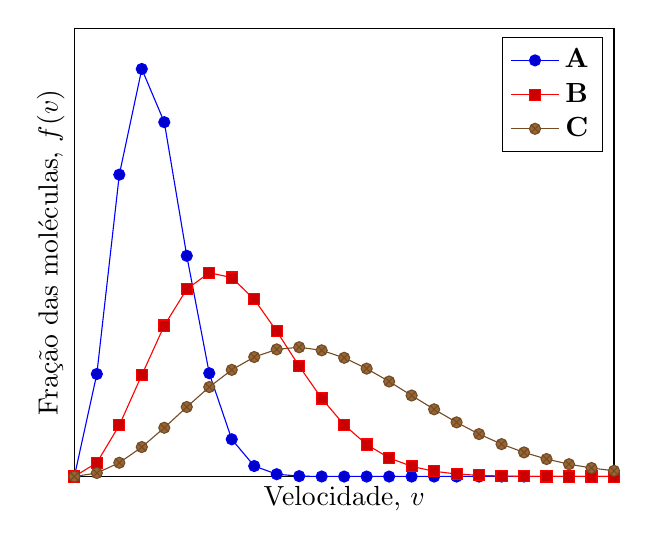
\begin{tikzpicture}
    \def\R{1000*8.314}% boltzmann constant
    \begin{axis}
        [
            domain = 0:2700,
            xlabel = {Velocidade, $v$},
            ylabel = {Fração das moléculas, $f(v)$},
            xtick=\empty, ytick=\empty,
            xmin=0, ymin=0,
            xmax=2700,
        ]
    \pgfplotsinvokeforeach{40,10,4} % Ar, Ne, He
    {
        \addplot
        {
            sqrt(2/pi)*(#1/(\R*298))^(3/2)*x^2*exp(-#1/(\R*298)*x^2/2)
        };
        % \addlegendentryexpanded{$#1$}
    }
    \legend{\ce{\textbf{A}},\ce{\textbf{B}},\ce{\textbf{C}}}
\end{axis}
\end{tikzpicture}